\documentclass[12pt]{article}

\usepackage[utf8]{inputenc}
\usepackage[T1]{fontenc}
\usepackage[spanish]{babel}
\usepackage{graphicx}
\usepackage{listings}
\usepackage{caption}
\usepackage{subcaption}
\usepackage[right=2cm,left=2cm,top=2cm,bottom=2cm]{geometry}
\usepackage{hyperref}
\usepackage{fancyhdr}
\usepackage{color}
\usepackage[export]{adjustbox}
\usepackage{graphicx}
\usepackage{float}
\usepackage{changepage}
\usepackage{multicol}
\usepackage{imakeidx}
\usepackage[spanish]{babel}
\usepackage[backend=biber]{biblatex}

\pagestyle{fancy}
\renewcommand{\footrulewidth}{0.4pt}
\setlength{\headheight}{15pt}


\fancyhead[L]{ CEIABD – MIA }
\fancyhead[R]{ Páez Anguita, Víctor }
\fancyfoot[L]{IES Gran Capitán}


\begin{document}

\begin{titlepage}
    \begin{center}
      \Large \bfseries{}
    \end{center}
    \vspace{0.1cm}
    \begin{center}
      \Large \bfseries{}
    \end{center}
    \vspace{0.1cm}
    \begin{center}
     \Large \bfseries{Algoritmos de búsqueda Evolutivos y de A*}
    \end{center}
    \vspace{0.0001cm}
    \begin{center}
        Departamento de informática \\ I.E.S. Gran Capitán - Córdoba
    \end{center}
        \vspace{2 cm}
\begin{figure}[h!]
    \centering
    
\includegraphics[width=.6\textwidth]{Portada.jpg}
    \label{fig:my_label}
\end{figure}
    \vspace{0.2 cm}
    \begin{center}
        Inteligencia artificial y Big data \\ Córdoba, 28 de Octubre 2024
    \end{center}
    \vspace{4 cm}
\null\hfill \textbf{Desarrollado por:}
\\
\\
\null\hfill Víctor Páez Anguita
\clearpage
\end{titlepage}

%%%%%%%%%%%%%%%%%%%%%%%%%%%Index%%%%%%%%%%%%%%%%%%%%%%%%%%%%%%%%
\tableofcontents
\clearpage
%%%%%%%%%%%%%%%%%%%%%%%%%%%Index%%%%%%%%%%%%%%%%%%%%%%%%%%%%%%%%

\section{Introducción}
Los algoritmos de búsqueda Evolutivos y el algoritmo A* son técnicas de búsqueda utilizadas en Inteligencia Artificial (IA) y 
otras áreas para resolver problemas de optimización y búsqueda de soluciones en espacios grandes o complejos.

\section{algoritmos de búsqueda Evolutivos}

Los algoritmos evolutivos son un grupo de algoritmos de optimización que se basan en principios de la evolución biológica, como la selección natural, 
la mutación y el cruce. La idea principal es generar una población inicial de posibles soluciones, evaluar su desempeño (o "fitness") y luego seleccionar y 
combinar las mejores para crear una nueva generación. Este proceso se repite, con mutaciones y combinaciones aleatorias, hasta que se encuentra una solución adecuada 
o se alcanza un límite de iteraciones.

\subsection{Características}

\begin{itemize}
    \item Población de soluciones: En vez de trabajar con una sola solución, manejan múltiples soluciones (población).
    \item Mutación y cruce: Usan operadores de mutación y cruce para introducir variabilidad y generar nuevas soluciones.
    \item Selección: Emplean algún mecanismo de selección para mantener las mejores soluciones.
\end{itemize}

\subsection{Aplicaciones en IA}

Los algoritmos evolutivos son muy usados en problemas donde el espacio de búsqueda es grande o no hay una función clara de optimización, 
como en el diseño de redes neuronales, optimización de parámetros, planificación automática y en sistemas de IA adaptativos.

\subsection{Beneficios}

\begin{itemize}
    \item Mayor flexibilidad. Los conceptos de algoritmo evolutivo se pueden modificar y adaptar para resolver los problemas humanos más complejos y cumplir con los objetivos establecidos.
    \item Mejor optimización. Se consideran todas las soluciones posibles. Esto significa que el algortimo no se limita una solución en particular.
    \item Soluciones ilimitadas. A diferencia de los métodos clásicos que presentan una única solución, los algoritmos evolutivos incluyen y ofrecen múltiples posibles soluciones a un problema.
\end{itemize}

\subsection{Tipos}

En la siguiente tabla podemos ver observar los tipos de algoritmos evolutivos más comunes:

\begin{figure}[h!]
    \centering
    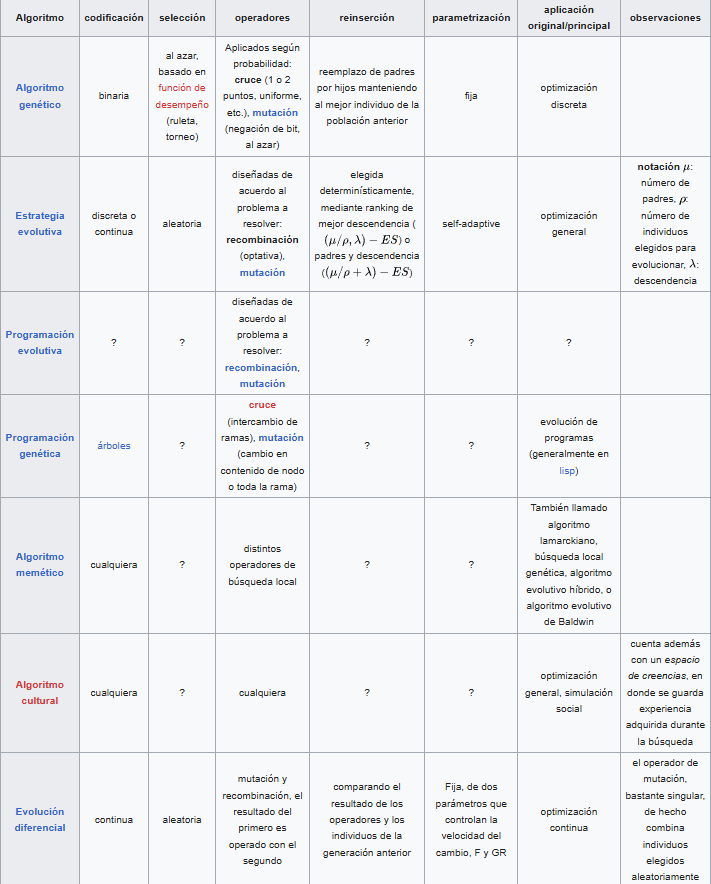
\includegraphics[width=.8\textwidth]{tablaevolutiva.PNG}
    \label{fig:my_label}
\end{figure}

\clearpage

\section{Algoritmo A*}

El algoritmo A* es una técnica de búsqueda heurística, ideal para encontrar el camino más corto en un grafo, lo que lo hace útil para resolver problemas de búsqueda de ruta. 
A* combina la búsqueda de costo uniforme (usando una función de costo g(n), que mide la distancia desde el punto de partida al nodo actual) con una heurística h(n) 
(estimación de la distancia restante al objetivo). El algoritmo evalúa cada nodo usando la función f(n) = g(n) + h(n), y se mueve hacia el nodo con el valor más bajo de f(n) 
para tratar de encontrar la ruta óptima.

\begin{figure}[h!]
    \centering
    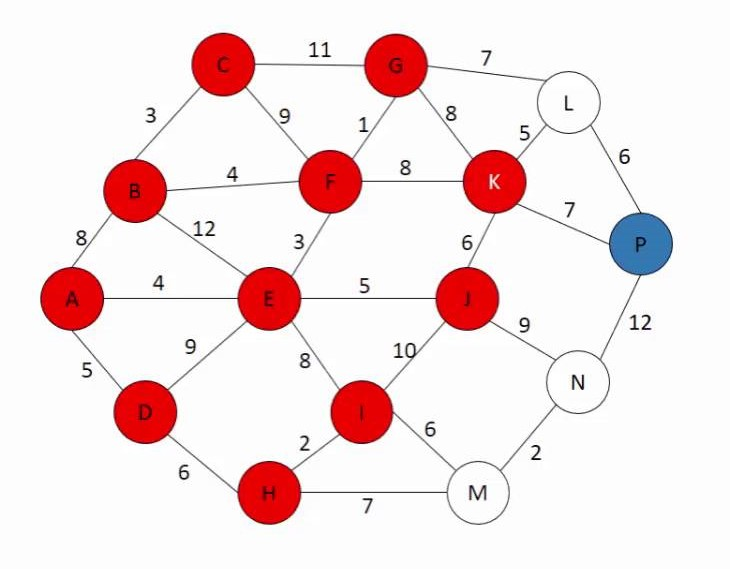
\includegraphics[width=.5\textwidth]{grafo.jpg}
    \label{fig:my_label}
\end{figure}

\subsection{Características}

\begin{itemize}
    \item Heurística: Utiliza una función heurística para guiar la búsqueda, lo cual puede hacerla muy eficiente.
    \item Óptimo y completo: Si la heurística es admisible (no sobreestima el costo), A* garantiza encontrar el camino óptimo.
    \item Flexibilidad: Puede ajustarse mediante diferentes heurísticas según el problema.
\end{itemize}

\subsection{Aplicaciones en IA}

A* es muy popular en la planificación de rutas y navegación de robots, videojuegos (para encontrar rutas entre puntos), 
y sistemas de planificación automatizada. Es ideal en situaciones donde se necesita un camino óptimo y se conoce una buena estimación heurística.



\clearpage

\section{Bibliografia}
\begin{itemize}
    \item \href{https://www.cognizant.com/es/es/glossary/evolutionary-algorithm#:~:text=Un%20algoritmo%20evolutivo%20es%20una,la%20reproducci%C3%B3n%2C%20mutaci%C3%B3n%20y%20recombinaci%C3%B3n.}{Cognizant}.
    \item \href{https://es.wikipedia.org/wiki/Algoritmo_evolutivo}{wikipedia}.
    \item \href{https://theblackboxlab.com/2020/06/22/que-son-los-algoritmos-evolutivos-y-para-que-se-usan/}{theblackboxlab}.
    \item \href{https://es.wikipedia.org/wiki/Algoritmo_de_b%C3%BAsqueda_A*}{wikipedia}.
    \item \href{https://aeia.home.blog/algoritmo-a-estrellas-a/}{aeia}.
    \item \href{https://escarbandocodigo.wordpress.com/2011/07/11/1051/}{escarbandocodigo}.

\end{itemize}

\end{document}
